\documentclass[dvipdfmx]{jarticle}
\usepackage[dvipdfmx]{graphicx}
\usepackage{tikz}
\usetikzlibrary{positioning, intersections, calc, arrows.meta, math, through}
\usepackage{tcolorbox}
\tcbuselibrary{theorems,breakable}
\usepackage{enumerate}
\newtcbtheorem[]{reidai}{例題}
{fonttitle=\gtfamily\sffamily\bfseries\upshape\large,
colframe=black,colback=black!15!white,
rightrule=1pt,leftrule=1pt,bottomrule=2pt,
colbacktitle=black,theorem style=standard,breakable,arc=10pt}
{tha}
\newcommand{\kai}%解答
{\noindent
\begin{tikzpicture}[scale=0.2, baseline=2.8pt]
\draw (3.3,1) node{\large\textgt{解 答}};
\draw[thick, rounded corners=3pt,] (0,0)--(6.5,0)--(6.5,2.2)--(0,2.2)--cycle;
\end{tikzpicture}\;}
\newcommand{\shomei}%証明
{\noindent
\begin{tikzpicture}[scale=0.2, baseline=2.8pt]
\draw (3.3,1) node{\textgt{証 明}};
\draw[double,thick,rounded corners=3pt,] (0,0)--(6.5,0)--(6.5,2.2)--(0,2.2)--cycle;
\end{tikzpicture}\;}
%補足
\newcommand{\hosoku}{\noindent
\begin{tikzpicture}[scale=0.2, baseline=2.8pt]
\draw (6,1) node{\large\textgt{補足}};
\fill (0,1)--(1,0)--(2,1)--(1,2)--cycle;
\fill[gray] (1,1)--(2,0)--(3,1)--(2,2)--cycle;
\fill (2,1)--(3,0)--(4,1)--(3,2)--cycle;
\fill (10,1)--(11,0)--(12,1)--(11,2)--cycle;
\fill[gray] (9,1)--(10,0)--(11,1)--(10,2)--cycle;
\fill (8,1)--(9,0)--(10,1)--(9,2)--cycle;
\end{tikzpicture}\;}
%注意
\newcommand{\chui}{\noindent
\begin{tikzpicture}[scale=0.2, baseline=2.8pt]
\fill (0,0)--(6.5,0)--(6.5,2.2)--(0,2.2);
\draw (3.3,1) node[white]{\large\textgt{注意!}};
\draw[thick] (0,0)--(6.5,0)--(6.5,2.2)--(0,2.2)--cycle;
\end{tikzpicture}\;}

\begin{document}
\begin{reidai}{2次方程式}{}
  次の2次方程式を解け。\vspace{-8pt}
  \begin{enumerate}[(1)\;]
    \item $x^2=1$
    \item $x^2-4x+1=0$
  \end{enumerate}
\end{reidai}
\vskip\baselineskip

\begin{reidai}{2次不等式}{}
  次の2次不等式を解け。\vspace{-8pt}
  \begin{enumerate}[(1)\;]
    \item $x^2 \geq 4$
    \item $x^2-4x+1 < 0$
  \end{enumerate}
\end{reidai}
\vskip\baselineskip

\kai ここは解答欄です。解答はここに書いてください。
\vskip\baselineskip
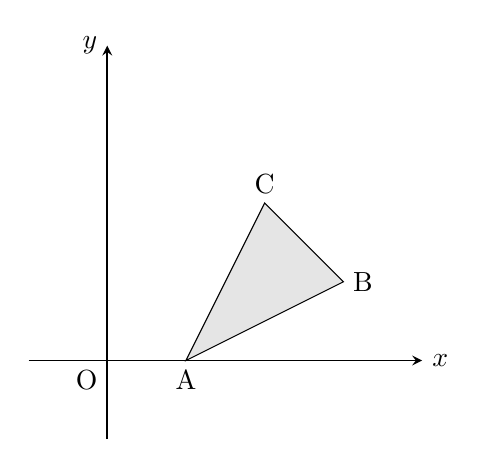
\begin{tikzpicture}[scale=1]
\coordinate[label=below:A] (A) at (1,0);
\coordinate[label=right:B] (B) at (3,1);
\coordinate[label=above:C] (C) at (2,2);
\filldraw[fill=gray!20!white] (A)--(B)--(C)--cycle;
\draw[->,>=stealth,semithick] (-1,0)--(4,0) node[right]{$x$};
\draw[->,>=stealth,semithick] (0,-1)--(0,4) node[left]{$y$};
\draw(0,0) node[below left]{O};
\end{tikzpicture}
\vskip\baselineskip

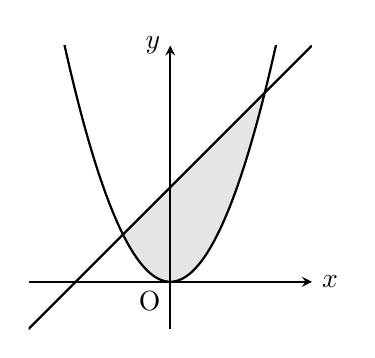
\begin{tikzpicture}[samples=200,scale=0.6]
\begin{scope}\clip (-3,-1) rectangle (3,5);
\fill[gray!20!white] plot[domain=-1:2](\x,{pow(\x,2)});
\draw[thick] plot(\x,{pow(\x,2)});
\draw[thick] plot(\x,\x+2);
\end{scope}
\draw[->,>=stealth,semithick] (-3,0)--(3,0)node[right]{$x$};
\draw[->,>=stealth,semithick] (0,-1)--(0,5)node[left]{$y$};
\draw (0,0)node[below left]{O};
\end{tikzpicture}

\end{document}



